% !TEX program = xelatex
% One-page A4 summary — generated by paper/make_position18_summary.py (all numbers read from artifacts).
\documentclass[10pt,a4paper]{ctexart}
\usepackage[margin=1.1cm]{geometry}
\usepackage{graphicx,booktabs,array,xcolor,amsmath}
\usepackage[hidelinks]{hyperref}
\setlength{\parindent}{0pt}\setlength{\parskip}{1.5pt}
\sloppy
\pagestyle{empty}
\definecolor{acc}{HTML}{1F4E79}
\definecolor{soft}{HTML}{F2F5F8}
\definecolor{warn}{HTML}{B03A2E}
\newcommand{\bd}[1]{\fontsize{8.5}{10.2}\selectfont\textbf{#1}}
\newcommand{\bt}[1]{\fontsize{8.5}{10.2}\selectfont #1}
\newcommand{\sm}[1]{\fontsize{7.5}{9.0}\selectfont #1}
\begin{document}
\enlargethispage{0.8cm}

{\color{acc}\fontsize{18}{21}\selectfont\bfseries AI-discovered candidate sequence factor at sgRNA position 18}\\[1pt]
{\fontsize{10}{12}\selectfont\itshape Multi-model attribution and cell-line-dependent evidence from the DeepCRISPR case study}\\[1pt]
\sm{Computational discovery summary for supervisor discussion $\cdot$ Status: computational discovery completed; experimental validation proposed（计算发现已完成，实验验证方案待评估）}\\[1.5pt]
{\color{acc}\hrule height 0.8pt}
\vspace{1.5pt}

\begin{minipage}[t]{0.44\textwidth}
{\color{acc}\bd{1. What we found}}\\[1pt]
\bd{Multiple model classes consistently identify the PAM-proximal region (positions 17--20) as a high-attribution region, with position 18 repeatedly emerging as a peak position.}\\[1.5pt]
\bt{多模型归因一致指向 PAM 邻近区域（17--20 位），第 18 位在多个模型与多个细胞系中重复成为峰值位置。}\\[1.5pt]
\sm{\itshape Attribution reflects model-derived importance and does not establish causality.}\\[2pt]
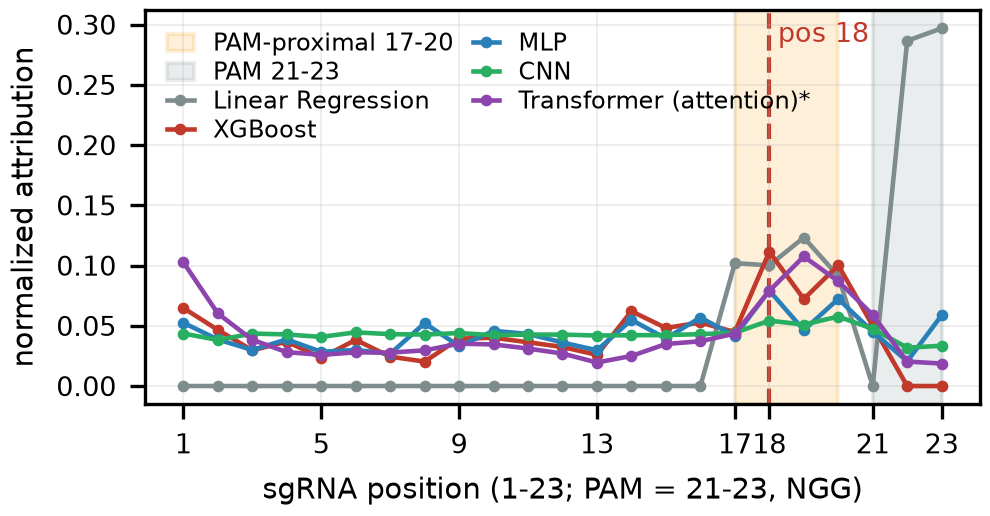
\includegraphics[width=\linewidth]{figures/position18_attribution.png}\\[1pt]
\sm{\textbf{Figure 1.} Normalized position attribution of five model classes (mean over cell lines; single-cell-line split). *Transformer = \emph{attention weight}, not gradient/tree attribution. Red dashed: position 18; orange: 17--20; grey: PAM 21--23.}
\end{minipage}\hfill
\begin{minipage}[t]{0.54\textwidth}
{\color{acc}\bd{2. Independent evidence}}\\[1pt]
\sm{
\begin{tabular}{@{}p{0.30\linewidth}p{0.66\linewidth}@{}}
\toprule
\textbf{Evidence} & \textbf{Result (from artifacts)}\\
\midrule
PAM-proximal region & highest-attribution region for CNN, MLP, XGBoost, Transformer\\
Position 18 & recurrent peak in HCT116 and HeLa across models\\
Profile correlation & mean pairwise Spearman 0.28--0.61 (23 positions)\\
Top-3 overlap & 0.30--0.53 of top-3 positions shared between models\\
Model classes & attention peaks at positions 1--2 in HCT116/HeLa (supporting only)\\
\bottomrule
\end{tabular}}
\\[2pt]
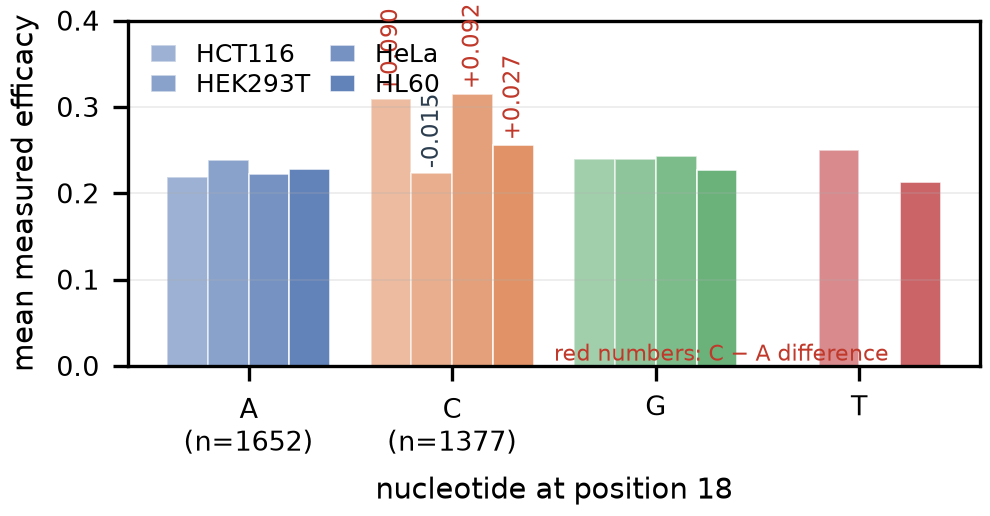
\includegraphics[width=\linewidth]{figures/position18_base_effect.png}\\[1pt]
\sm{\textbf{Figure 2.} Mean measured editing efficiency by the nucleotide at position 18 (n = 495--3\,278 per bar); numbers: C $-$ A difference.}\\[1.5pt]
{\color{acc}\bd{The position-18 nucleotide effect is context-dependent rather than universal.}}\\[1pt]
\bt{第 18 位碱基与编辑效率的关系具有明显细胞背景依赖性（HCT116/HeLa 中 C 高于 A，HL60 差异缩小，HEK293T 方向反转），更适合作为 context-dependent candidate factor。}
\end{minipage}

\vspace{2pt}
\colorbox{soft}{\begin{minipage}{\dimexpr\textwidth-2\fboxsep\relax}
{\color{acc}\bd{3. Current interpretation}}\\[1pt]
\bt{Position 18 is a \textbf{candidate sequence-associated factor} whose predictive importance is repeatedly identified by multiple model classes, while its base-specific efficacy association varies across cell-line contexts. 第 18 位目前可定义为一个候选序列相关因素。\quad\textbf{This is an association / model-attribution finding, not a causal conclusion.}}\\[1.5pt]
\sm{\bfseries Why this candidate?} \sm{\textbf{01} PAM-proximal 17--20 is the highest-attribution region for CNN, MLP, XGBoost and Transformer；\textbf{02} position 18 is the modal peak in HCT116 and HeLa；\textbf{03} measured C $-$ A difference HCT116 +0.090, HeLa +0.092, HL60 +0.027, HEK293T -0.015（方向随细胞系改变）。}\\[1pt]
\sm{\itshape Evidence chain: multi-model attribution $\rightarrow$ PAM-proximal region $\rightarrow$ position 18 repeatedly prioritized $\rightarrow$ base-specific efficacy differences $\rightarrow$ cell-line-dependent pattern $\rightarrow$ candidate sequence factor.}
\end{minipage}}
\vspace{2pt}

{\color{acc}\bd{4. Minimal experimental validation (proposed, not yet performed)}}\\[1pt]
\begin{minipage}[t]{0.40\textwidth}
\bt{\textbf{Test whether perturbing the model-prioritized nucleotide at position 18 reproducibly changes Cas9 editing efficiency.}}\\[1pt]
\sm{WT: position 18 = original C\\
\hspace{1em}$\vdash$ C$\rightarrow$A \quad $\vdash$ C$\rightarrow$G \quad $\vdash$ C$\rightarrow$T\\
Keep the remaining sgRNA sequence unchanged.\\
Compare measured editing efficiency of each variant with WT.\\
Controls: WT $+$ variants $+$ negative control $+$ reference/positive control.}
\end{minipage}\hfill
\begin{minipage}[t]{0.575\textwidth}
\sm{\bfseries Freeze the prediction before the experiment (prospective test):} \sm{AI prediction (positional importance from ISM / IG / SHAP) $\rightarrow$ freeze hypothesis (position and variant set) $\rightarrow$ wet-lab experiment (WT vs variants, efficiency readout) $\rightarrow$ compare prediction with observation.}\\[1.5pt]
\sm{\color{warn}Directional mutation prediction is currently unavailable: all CNN ISM / IG / SHAP / attention outputs are unsigned magnitudes (only linear coefficients carry a sign, and they diverged in 56/192 runs). Only \emph{positional importance} is supported, so the pre-registered hypothesis specifies the position and variant set, not a predicted direction.}
\end{minipage}

\vspace{2pt}
{\color{acc}\hrule height 0.5pt}
\vspace{1pt}
\sm{\bfseries Limitations:} \sm{computational/observational evidence only; position and nucleotide-specific effects are not fully separable; cell-line differences may reflect sequence composition or cohort differences (position-18 T occurs mainly in HEK293T/HL60); wet-lab validation not yet performed.}\\[1pt]
\sm{\bfseries Sources:} \sm{\texttt{attribution\_summary.csv}, \texttt{position18\_efficacy\_by\_base.csv}, \texttt{cross\_model\_position\_consistency.csv}, \texttt{cellline\_effects.csv}, \texttt{evidence\_matrix.csv}; PAM 21--23 (NGG) verified from raw sequences. \quad\bfseries Status: computational discovery completed; validation proposed（计算发现已完成）\quad Contact: \_\_\_\_\_\_}
\end{document}
